\chapter{Разработка оптимизаций}\label{ch:ch2}

В этой главе описаны разработанные оптимизации. Не все представленные оптимизации были приняты сообществом openEulerGCC \footnote{https://gitee.com/src-openeuler/gcc/} по разным причинам. Некоторые из описанных далее оптимизаций будут представлены сообществу позднее, а некоторые, возможно, будут заменены другими подходами. Тем не менее автор считает, что исследованные подходы также представляют научный интерес.


\section{Улучшение существующих оптимизаций}\label{sec:ch2/sect1}
\todo{ Написать введение}
\subsection{Преобразование условных переходов} \label{opt:ifconv}
Преобразование условных переходов (If-conversion) — это хорошо известный метод оптимизации, который заменяет инструкцию перехода и зависящий от него поток управления, предикатным исполнением, соединяя тем самым две различные ветки потока управления в одну для последующего совместного исполнения.  В результате целевой код содержит меньшее количество инструкций перехода, что снижает нагрузку на аппаратный предсказатель переходов, однако такой подход позволяет увеличить количество избыточных инструкций во время исполнения \cite{bruel2021if}. Обычно эта оптимизация основана на представлении SSA, однако в компиляторе GCC используется другой подход. На этом этапе SSA форма отсутствует, что может привести к следующей проблеме (рис. \ref{fig:ifcvtsvg1}): если в одной из ветвей исполнения в качестве регистра назначения используется  тот же регистр (reg1 на
Рисунке \ref{fig:ifcvtsvg1}), что в другом в качестве источника, то после слияния будет создано неправильное определение reg1.

Предлагаемое решение содержит принудительное переименование регистров. Такая трансформация была добавлена при коллизии такого типа. Регистры коллизий определяются как:

$$rename\_candidates = DEFS_{left\_bb} \cap USES_{right\_bb} $$
Если $rename\_candidates[i]$ все еще жив в конце базового блока $BB$, то трансформация не может быть применена.


\begin{figure}[htbp]
	\centering

	\includesvg[width = 400pt, inkscapelatex=false ]{SVG/ifcvt-1.svg}
	\caption{Пример некорректного преобразования условных переходов в следствие отсутствия SSA формы.}
	\label{fig:ifcvtsvg1}
\end{figure}

Улучшение преобразования условных переходов в компиляторе GCC было размещено под опцией \mbox{\textbf{-fifcvt-allow-register-renaming}}. Такой подход помогает уменьшить количество "хвостовых"\   базовых блоков в целевых тестах. (Листинг \ref{ifcvtcode1}). Такие базовые блоки были обнаружены путем применения технологии профилирования из главы \ref{p1:optop:profile}. Сбор событий при помощи PMU показывал повышенное количество задержек во фортн-энде (front-end) процессора. Причиной этих задержек оказались постоянный переходы в "хвостовые"\   базовые блоки и обратно.


\begin{ListingEnv}[!h]
	\captiondelim{ } % разделитель идентификатора с номером от наименования
		\caption{Пример "хвостовых"\  базовых блоков, которые будут оптимизированы предложенным улучшением преобразования условных переходов.}
	\label{ifcvtcode1}
	\begin{Verb}
		4145bc:   ret
		4145c0:   mov     x5, #0x100000000              
		4145c4:   add     x7, x7, x5
		4145c8:   b       4131d0
		4145cc:   mov     x2, #0x100000000               
		4145d0:   add     x6, x6, x2
		4145d4:   b       4145a0 
		4145d8:   mov     x3, #0x100000000                
		4145dc:   add     x11, x11, x3
		4145e0:   b       41454c
		4145e4:   mov     x3, #0x100000000 
		4145e8:   add     x11, x11, x3
		4145ec:   b       4144fc 
	\end{Verb}
\end{ListingEnv}

Конечно же применение подобной трансформации сопряжено с определенными рисками уменьшения производительности. Повсеместное преобразование может привести к увеличенному давлению на регистровый файл, что в свою очередь приводит к излишнему использованию стека. Поэтому вводятся функции стоимости для данной оптимизации: главным, однако далеко не единственным критерием применения преобразования условных переходов является итоговый размер базового блока, в  разработанной модели, этот параметр может задаваться пользователем, однако на исследуемой машине эмпирически был выведен  ограничивающий размер  результирующего базового блока равный 48 инструкций.
\begin{ListingEnv}[!h]
	\captiondelim{ } % разделитель идентификатора с номером от наименования
	\caption{Образец проверки из теста povray (трассировка лучей).}
	\label{ifcvtcode2}
	\begin{Verb}
		if (lf == 0.0 || lf * f < 0)
		{
			changes++;
		} 
	\end{Verb}
\end{ListingEnv}


\begin{ListingEnv}[!h]
	\captiondelim{ } % разделитель идентификатора с номером от наименования
	\caption{Листинг \ref{ifcvtcode2} в представлении GIMPLE GCC.}
	\label{ifcvtcode3}
	\begin{Verb}
		<bb 9> [local count: 118111600]:
		if (lf_11 == 0.0)
		goto <bb 11>; [50.00%]
		else
		goto <bb 10>; [50.00%]
		
		<bb 10> [local count: 59055800]:
		_5 = lf_11 * val_42;
		if (_5 < 0.0)
		goto <bb 11>; [41.00%]
		else
		goto <bb 12>; [59.00%]
		
		<bb 11> [local count: 83268678]:
		changes_22 = changes_10 + 1;
		
		<bb 12> [local count: 118111600]:
		# changes_9 = PHI <changes_10(10), changes_22(11)>
	\end{Verb}
\end{ListingEnv}
В качестве примера дополнительных ограничений рассмотрим оптимизацию участка кода из теста povray (трассировка лучей). В одном из основных горячих циклов можно встретить следующую проверку, изображенную на листинге \ref{ifcvtcode2}. В GCC этот код трансформируется в следующий набор базовых блоков (Листниг \ref{ifcvtcode3}) Операция умножения считается достаточно тяжелой, по этому преобразование ее в  один базовый блок вместе с простым сравнением с нулем кажется компилятору неэффективным, однако было обнаружено, что для конкретной исследуемой платформы такое преобразование все же увеличивает итоговую производительность программы.  



\begin{ListingEnv}[!h]
	\captiondelim{ } % разделитель идентификатора с номером от наименования
	\caption{Листинг \ref{ifcvtcode3} в представлении GIMPLE GCC после оптимизации преобразования условных переходов.}
	\label{ifcvtcode4}
	\begin{Verb}
		<bb 9> [local count: 118111600]:
		_5 = lf_11 * val_42;
		_36 = _5 < 0.0;
		_51 = lf_11 == 0.0;
		_18 = _36 | _51;
		if (_18 != 0)
		goto <bb 10>; [70.50%]
		else
		goto <bb 11>; [29.50%]
		
		<bb 10> [local count: 83268678]:
		changes_22 = changes_10 + 1;
		
		<bb 11> [local count: 118111600]:
		# changes_9 = PHI <changes_10(9), changes_22(10)>
	\end{Verb}
\end{ListingEnv}

Оптимизация реализована в проходе ifcombine на этапе  Gimple. Следующее преобразование было введено для оптимизации целевого кода  и оно основано на том факте, что некоторые инструкции быстрее (или дешевле с точки зрения времени), чем условные переходы (рисунок \ref{ifcvt2svg1}). Это означает, что объединение двух сравнений в рамках операции AND или OR в один базовый блок, чтобы не выполнять «ленивое» вычисление булевого оператора, является более эффективным. Реализация gcc по умолчанию объединяет текущее сравнение со следующим, только если оно является условным. Эта оптимизация определяет список дешевых gimple-assign-insns, которые также могут быть объединены в один базовый блок в этом проходе.

\begin{figure}[htbp]
	\centering
	\includesvg[width = 400pt, inkscapelatex=false ]{SVG/ifcvt2.drawio.svg}
	\caption{Схема улучшения стоимостной эвристики в оптимизации преобразования условных переходов.}
	\label{ifcvt2svg1}
\end{figure}

Введение дешевых инструкций и добавление туда умножения чисел с плавающей точкой позволяет в примере из листинга \ref{ifcvtcode3} объединить  базовый блок, содержащий сравнение float var с 0.0, c блоком с дешевой инструкцией умножения с плавающей точкой.Таким образом, один условный оператор goto и один базовый блок будут удалены. После этого преобразования оптимизированный фрагмент будет выглядеть следующим образом во внутреннем представлении компилятора GCC (Листинг \ref{ifcvtcode4}).

\subsection {Векторизация циклов с небольшим числом итераций}
Векторизация — это известный метод, использующий параллелизм данных \cite{nuzman2006autovectorization}. В ходе текущего исследования было обнаружено, что векторизация генерирует хвосты (т. е. векторизованный код для меньшего коэффициента векторизации), но не использует их, когда фактическое количество итераций равно коэффициенту векторизации хвоста ($VEC\_FACTOR$). Опять же, чтобы это увидеть пришлось воспользоваться техникой сэмплирующего профилирования из главы \ref{p1:optop:profile}, в ходе которой было обнаружено, что несмотря на включенную векторизацию, приложение все равно большую часть времени исполняла скалярную версию участка. Следовательно, когда $VEC\_FACTOR$ равен, например 8, код будет сгенерирован для $VEC\_FACTOR = 4$ и $VEC\_FACTOR = 2$. Если во время выполнения фактическое количество итераций будет только 4, то будет выбран скалярный вариант. Это небольшое и простое улучшение меняет условие пересечения указателя в заголовке цикла.

Рассмотрим простой цикл (Листинг \ref{algexample_1})

\begin{ListingEnv}[!h]
	\captiondelim{ } % разделитель идентификатора с номером от наименования
	\caption{Простой цикл рассматриваемый оптимизацией векторизации.}\label{algexample_1}
	\begin{Verb}
		\\ a,b,c: any arrays with size N
		for (i = 0; i<N; i+=1)
		    c[i] = a[i] *b[i]
	\end{Verb}
\end{ListingEnv}
GCC преобразует этот цикл в (Листинг \ref{vectorized_loop_example}), и легко видеть, что если, например, $c-a = VEC\_FACTOR/2$ и $N = VEC\_FACTOR/2$, то будет выбрана скалярная версия.

\begin{ListingEnv}[!h]
	\captiondelim{ } % разделитель идентификатора с номером от наименования
	\caption{Цикл (Листинг \ref{algexample_1}) после векторизации GCC}\label{vectorized_loop_example}

	\begin{Verb}

		\\ a,b,c: any arrays with size N
		VEC_FACTOR: factor estimated by GCC pass
		if  (abs (c - a) < VEC_FACTOR  ||  
		     abs (c - b) < VEC_FACTOR) 
		    goto SCALAR;

		if (N < VEC_FACTOR)
		    goto TAIL;
			
		for (i;i<N;i+=VEC_FACTOR)
		    WIDE_C = WIDE_A * WIDE_B 
		    \\ WIDE_X has VEC_FACTOR size 
			
		TAIL:
		if (i<N - VEC_FACTOR/2)
		    goto SCALAR;
			
		SEMIWIDE_C = SEMIWIDE_A * SEMIWIDE_B 
		\\ SEMIWIDE has VEC_FACTOR/2 size 
		
		SCALAR:
		for (i = 0; i<N; i+=1)
		    c[i] = a[i] *b[i]

	\end{Verb}
\end{ListingEnv}

\begin{ListingEnv}[!h]
	\captiondelim{ } % разделитель идентификатора с номером от наименования
	\caption{Модифицированная проверка для (Листинг \ref{vectorized_loop_example})}\label{replaced_check}
	
	\begin{Verb}
		
		
		\\ a,b,c: any arrays with size N
		\\ VEC_FACTOR: factor estimated by GCC pass
		if (abs (c - a) < min(VEC_FACTOR,N) ||
		    abs (c - b) < min(VEC_FACTOR,N)) 
		   goto SCALAR;
	\end{Verb}
\end{ListingEnv} 

Чтобы это исправить, предлагается простое решение: заменить строки 1 и 2 в векторизованной версии (Листинг \ref{vectorized_loop_example}) следующим кодом (Листинг \ref{replaced_check}). Добавлен параметр \textbf{--param=vect-alias-flexible-segment-len}. Эта оптимизация повышает производительность приложения x264.




\section{Шаблонные оптимизации}\label{sec:ch2/sect2}
\todo{ Написать введение}
\subsection{Оптимизация двойного умножения}
Оптимизация двойного умножения — это шаблонное преобразование компилятора, предназначенное для преобразования алгоритма 64-битного умножения в  эффективные инструкции. Таким образом, программа может лучше использовать возможности аппаратуры и повысить производительность всего приложения. Это стандартная архитектурно-зависимая оптимизация. Различные архитектуры предоставляют разные наборы команд. Иногда инструкции системы команд просты, что позволяет легко найти аналоги для любой архитектуры (например, инструкция add), но иногда, особенно в CISC-архитектурах, могут встречаться достаточно сложные инструкции, эквивалент которых потребует десятков и даже сотен команд.  \cite{bansal2021reduced, isen2009tale}.


Идея таких вычислений основана на максимальных значениях половинного умножения ($s$ - размер в битах).
\begin{equation*} \label{eq1}
	\left(2^{s/2}-1\right)^2=2^s-2^{s/2+1}+1<2^s-1
\end{equation*}

При разделении аргументов на части $s/2$ широкое умножение можно переписать как:
\begin{equation*} \label{eq2}
	\begin{split}
		res& =a\cdot b =\left(2^{s/2}a_{hi}+a_{lo}\right)\left(2^{s/2}b_{hi}+b_{lo}\right) \\
		& =2^sa_{hi}b_{hi}+2^{s/2}\left(a_{hi}b_{lo}+a_{lo}b_{hi}\right)+a_{lo}b_{lo}  
	\end{split}
\end{equation*}
Результат состоит из двух частей: младшей (от $1$ до $2^s - 1$) и старшей (от $2^s$ до $2^{2s} -1$). Первое слагаемое  и правая часть второго слагаемого станут старшей частью результата. левая часть второго и третьего слагаемых станут младшей частью результата.


\begin{equation*} \label{eq3}
	\begin{split}
		2^s\le2^sa_{hi}b_{hi}<2^{2s}
	\end{split}
\end{equation*}
\begin{equation*} \label{eq4}
	\begin{split}
		2^{s/2}& \le2^{s/2}\left(a_{hi}b_{lo}+a_{lo}b_{hi}\right)\\ 
		& \le2^{3s/2}\left(2^{s+1}-2^{s/2+2}+1\right)
	\end{split}
\end{equation*}
\begin{equation*} \label{eq5}
	\begin{split}
		1\le a_{lo}b_{lo}<2^s
	\end{split}
\end{equation*}
Несложно доказать, что сложения могут привести к переполнению во время этих вычислений. Переименуем слагаемые для лучшей читабельности:
\begin{equation*} \label{eq6}
	\begin{split}
		mid\_res&=a_{hi}b_{lo}+a_{lo}b_{hi} \\
		&=mid\_res\_real+mid\_res\_overflow
	\end{split}
\end{equation*}
\begin{equation*} \label{eq7}
	\begin{split}
		res_{lo}&=2^{s/2}mid\_res\_real_{lo}+a_{lo}b_{lo} \\
		&=res\_low\_real+res\_low\_overflow
	\end{split}
\end{equation*}

\begin{flalign*}  \label{eq8}
	res_{hi}&=middle\_res\_real_{hi}+a_{hi}b_{hi} \notag  \\
	&=res\_high\_real+\dfrac{res\_low\_overflow}{2^s}\\
	&\phantom{=res\_high\_real}+\dfrac{mid\_res\_overflow}{2^{s/2}} \notag 
\end{flalign*}



\begin{equation*} \label{eq9}
	res=2^s \cdot res_{hi}+res_{lo}
\end{equation*}

Все вычисления сопоставляются с использованием существующего механизма сопоставления шаблонов GCC и преобразуются в одиночные умножения более широких типов. Количество инструкций значительно уменьшено. На CPUBench наблюдалось улучшение производительности в 30 \% на тесте OpenSSL.

\subsection{Шаблонная криптография}
В этом разделе поднимается важная тема для различных встраиваемых устройств и расширений архитектуры. В современном мире существует множество специализированных устройств для конкретных задач; например, ускорители для нейронных сетей \cite{chen2020survey}, для научных вычислений \cite{weber2010comparing}, для обработки графов \cite{rahman2020graphpulse} и т. д.

В недавнем исследовании \cite{peccerillo2022survey} Pecceriilo et al., 2022, классифицировали около 100 различных типов
ускорителей. Таким образом, в этой тенденции компилятор становится очень практичным инструментом, который может компилировать (потенциально автоматически) и планировать выполнение задач на разных устройствах. В настоящее время разные компании пытаются разработать собственный подход к решению этой задачи \cite{tavarageri2019automatic,chen2022case,kovac2022towards}.

Небольшая часть этой глобальной проблемы была решена в ходе нынешнего исследования. Kunpeng 920 имеет на плате расширение криптографии, которое включает специальные инструкции для crc32 и AES. Их можно использовать напрямую через встроенный язык ассемблера или встроенные функции компилятора. Добавлены оптимизации компилятора, которые могут определять возможность использования инструкций в соответствии с семантикой кода.

Оптимизация соотносит весь алгоритмам, включая предварительно рассчитанные таблицы, и статически проверяет, что все предварительно рассчитанные таблицы не изменяются во время выполнения. Оптимизация контролируется флагами \textbf{-fcrypto-accel-aes} и \textbf{-fcrypto-accel-crc32}. Оба шаблона были реализованы внутри RTL, поскольку они являются  архитектурно-зависимыми. На верхнем уровне логика оптимизаций очень похожа друг на друга. Следующие шаги описывают преобразование шаблона AES:

\begin{enumerate}
	\item \textbf{Сбор ссылок на таблицы AES}: Разработан оптимизационных проход внутри компилятора GCC для поиска ссылки на соответствующие таблицы шифрования/дешифрования AES. Такие инструкции являются отправной точкой для дальнейшего анализа.
	\item \textbf{Формирование раундов AES}: Анализируются ссылки на таблицы и собираются инструкции, выполняющие вычисления, относящиеся к AES. связывая их вместе в блоки и раунды.
	\item \textbf{Проверка шаблона AES}: Анализируются раунды и связываются вместе.
	\item \textbf{Генерация кода AES}: Генерируется код AES для всех найденных раундов.
\end{enumerate}

Для сопоставления внутреннего представления компилятора на уровне RTL использовался собственные шаблонный анализатор.Механизм сопоставления был создан на основе существующих генераторов сопоставлений match.pd GENERIC и GIMPLE.  Код для необходимой проверки шаблона генерируется во время компиляции GCC. Анализатор генерирует заранее упорядоченную последовательность аргументов.


Специальные инструкции сократили общее количество инструкций в целевых горячих циклах, что привело к значительному ускорению. Улучшение производительности на 10+ \% было достигнуто на
тестах openSSL и gzip.

К сожалению, оптимизация crc32 не была принята, поскольку менее общая оптимизация, обеспечивающая большую производительность при использовании gzip, была предложена другими авторами.

\subsection{Шаблонная подстановка инструкций}

Одной из основных основных задачей компилятора является выбор наиболее подходящих инструкций, которыми можно будет наиболее лаконично и в то же время оптимально с точки зрения производительности выразить внутреннее представление программы \cite{blindell2016instruction}. В данной работе  не изменяется работа стандартного прохода выбора инструкций, однако добавляется несколько небольших шаблонов, который способствуют лучшей утилизации набора команд архитектуры ARM64.

Так, арифметическое выражение вида 
\begin{flalign*}  \label{eq10}
	B = (((A &>> 15) \& 0x00010001) << 16) -\\
	((A &>> 15) \& 0x00010001)
\end{flalign*}

до внесенных изменений транслировалось в векторной версии в (Листинг \ref{unoptimal1}) может быть транслировано в (Листинг  \ref{optimal1})
\begin{ListingEnv}[!h]
	\captiondelim{ } % разделитель идентификатора с номером от наименования
	\caption{Пример неоптимального выбора инструкций №1}\label{unoptimal1}
	
	\begin{Verb}
			xtn v18.4h, v17.4s
			xtn2 v18.8h, v1.4
	\end{Verb}
\end{ListingEnv} 
\begin{ListingEnv}[!h]
	\captiondelim{ } % разделитель идентификатора с номером от наименования
	\caption{Оптимальный выбор инструкций для Листинга \ref{unoptimal1} }\label{optimal1}
	\begin{Verb}
			uzp1 v17.8h, v18.8h, v17.8h
	\end{Verb}
\end{ListingEnv} 

Таким  же методом был преобразован код  (Листинг \ref{unoptimal2}) в более оптимальную версию, использующую инструкции smin/smax на (Листинг \ref{optimal2})
\begin{ListingEnv}[!h]
	\captiondelim{ } % разделитель идентификатора с номером от наименования
	\caption{Пример не оптимального выбора инструкций №2 }\label{unoptimal2}
	\begin{Verb}
			sshr v1.4s, v1.4s, #10
			neg v24.4s, v1.4s
			mov v20.16b, v1.16b
			sshr v24.4s, v24.4s, #31
			bic v20.4s, #0xff
			cmeq v20.4s, v20.4s, #0
			bif v1.16b, v24.16b, v20.16b
	\end{Verb}
\end{ListingEnv} 
\begin{ListingEnv}[!h]
	\captiondelim{ } % разделитель идентификатора с номером от наименования
	\caption{Оптимальный выбор инструкций для Листинга \ref{unoptimal2} }\label{optimal2}
	\begin{Verb}
		movi v2.2d, #0x0 // (outside the loop)
		movi v3.2d, #0xff000000ff // (outside the loop)
		...
		smax v18.4s, v18.4s, v2.4s // (inside the loop)
		smin v18.4s, v18.4s, v3.4s // (inside the loop)
		uzp1 v17.8h, v18.8h, v17.8h
	\end{Verb}
\end{ListingEnv} 



\section {Девиртуализация} \label{opt:devirt}

Современные языки программирования с высоким уровнем абстракции, такие как Java, С++ и C\#, используют динамические таблицы вызовов для реализации полиморфизма. \cite{calder1994quantifying,suganuma2000overview,bauer2021novt} В этой схеме адрес вызываемой функции определяется только во время выполнения программы. Виртуальные функции в объектно-ориентированных языках программирования являются одним из основных источников косвенных переходов в программах. Также в языках C/C++ можно использовать указатели на функции, а в GCC доступны указатели на метки внутри программы \cite{shah1995function}. Такой метод программирования позволяет пользователю создавать косвенные вызовы и переходы. Однако нетривиальное выполнение инструкций управления может замедлить работу центрального процессора, так как для эффективной обработки инструкций управления суперскалярному процессору необходимо предсказывать целевой адрес перехода. Для этого используются специальные устройства-предсказатели \cite{mcfarling1993combining,mittal2019survey}. Однако, предсказание косвенного перехода отличается от предсказания условного, так как в первом случае конечных адресов может быть множество и их необходимо хранить в памяти предсказателя. Это может потребовать лишней площади на кристалле \cite{driesen1998accurate}. Существующие методы разработки аппаратуры позволяют использовать принцип виртуального счетчика инструкций, но такой подход все равно требует дополнительной логики непосредственно в аппаратуре \cite{redmond2007vpc}.

Текущие подходы к решению данной задачи в основном фокусируются на разрешении вызовов виртуальных функций для объектно-ориентированного программирования \cite{namolaru2006devirtualization,padlewski2017devirtualization}. Отсутствие информации о целевых функциях в графе вызова затрудняет межпроцедурные оптимизации и делает невозможной подстановку функций непосредственно в код, что существенно ограничивает оптимизационные возможности компилятора \cite{li2010lightweight,pande1996data}.


В статье \cite{chernonog2023статический} описывается два метода преобразования косвенных переходов: статический и динамический.  

Статический метод по своей сути является расширением стандартной методологии девиртуализации компилятора GCC. Его работа разделена на две части:

\begin{enumerate}
	\item \textbf{Анализ сигнатур функций}: Авторами предлагается анализировать сигнатуры функций для определений и вызовов. Если сигнатура вызываемой функции совпадает с сигнатурой определения то функция определения считается кандидатом.
	\item \textbf{Трансформация косвенного перехода}: На этом этапе, в случае единственного кандидата, косвенный вызов функции заменяется вызовом найденной процедуры. Если же кандидатов несколько, то приходится выстраивать цепочку сравнений адресов переходов. что не всегда является оптимальным
\end{enumerate}


\begin{figure}[ht]
	\centerfloat{
		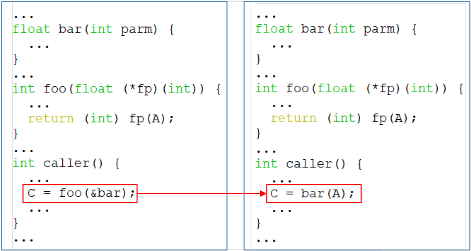
\includegraphics[scale=1]{PNG/ICP}
	}
	\caption{Пример замены косвенного вызова.}\label{fig:ICP1}
\end{figure}

С другой стороны динамический метод использует информацию, собранную во время выполнения программы \cite{baev2015profile,ishizaki2000study}, чтобы изменить косвенные переходы, не требуя повторной компиляции программы, как это происходит при использовании профилирования или системы JIT-компиляции (Just-in-Time compilation). Для решения этой проблемы предлагается встраивать средства трансформации кода непосредственно в исполняемую программу. В случае систем JIT перекомпилированный код отдельного метода или функции обычно помещается во вновь выделенный участок памяти \cite{cravvford1988study}. Однако здесь предлагается использовать единый участок памяти, изменяя его содержимое во время исполнения.

\textbf{Алгоритм}
 \begin{enumerate}
 	\item \textbf{Выбор косвенных переходов}: В ручном режиме в исходном коде программы  необходимо обернуть косвенный вызов или переход типа goto специальными библиотечными макро-определениями "DDL\_GOTO"\  или "DDL\_CALL". При использовании автоматического режима компилятор на основе графа вызовов принимает решение о применении оптимизации. 
 	\item \textbf{Трансформация косвенных переходов}: Вместо каждой инструкции перехода генерируется "окно"\  в виде заранее определенного количества nop инструкций и вызовов библиотечных функций сбора статистики и замены инструкций nop условными переходами при превышении счетчиков. Оригинальный косвенный переход несомненно сохраняется в самом конце.
 	\item \textbf{Запуск программы и сбор статистики}: Этот этап и все последующие  выполняются в ходе работы программы (и не требуют каких-либо действий со стороны пользователя или компилятора). Каждый раз, когда программа достигает модифицированного косвенного перехода, вызывается библиотечная функция для обновления статистики целевых адресов этого перехода. Библиотека  накапливает статистику отдельно для каждого перехода, который идентифицируется по уникальному номеру, присвоенному при инициализации.
 	\item \textbf{Трансформация в реальном времени}: Когда собранно достаточное количество статистической информации (которое задается параметром N), запускается функция модификации кода программы. Целевые адреса сортируются в порядке уменьшения количества совершенных по ним переходов. Если 95 \% переходов происходит не более чем по k адресам, то выполняется замена цепочки nop инструкций на условные переходы (листинг \ref{indirect_algo1}). В противном случае происходит вставка исходного косвенного перехода.
	\item \textbf{Работа оптимизированного перехода}: После преобразования перехода, режим сбора статистики целевых адресов отключается. Однако информация о количестве выполнений данного перехода продолжает накапливаться, а также записывается количество случаев, когда в преобразованном коде отсутствует прямой переход по полученному целевому адресу, и должен сработать первоначальный косвенный переход (который находится дальше по коду), то есть оптимизация для полученного адреса не произведена. Если количество пропущенных переходов станет значительным по сравнению с общим числом входов в данный участок кода, то цепочка прямых условных переходов будет заменена первоначальным блоком nop инструкций, и снова будет запущен сбор статистики. Другими словами, будет выполнен переход к шагу 2. При этом статистика адресов, собранная на предыдущем этапе выполнения шага 3, учитывается с коэффициентом 0.5, что позволяет сохранить эту информацию.
 \end{enumerate}

\begin{ListingEnv}[!h]
	\captiondelim{ } % разделитель идентификатора с номером от наименования
	\caption{Псевдокод преобразованного косвенного перехода}\label{indirect_algo1}
	
	\begin{Verb}
		
		INT entry_count = 0;
		entry_count++;
		START_REWRITE_POINT:
		NOP
		NOP
		...
		NOP // k-times reapeat
		BOOL collect_stat_mode = FALSE;
		INT miss_count = 0;
		miss_count++;
		if ( entry_count == N)
		&& (miss_count > entry_count >> 4) {
			if (!collect_stat_mode){
				collect_stat_mode = TRUE;
				CALL DDL_DISABLE_OPTIMIZATON();
			} else {
				miss_count = 0;
				entry_count = 1;
				CALL DDL_REWRITE_INDIRECT();
				collect_stat_mode = FALSE;
			}
		}
		if (collect_stat_mode) {
			CALL DDL_UPATE_STATISTICS();
		}
		goto *addr; // original indirect branch
		
	\end{Verb}
\end{ListingEnv} 


\begin{ListingEnv}[!h]
	\captiondelim{ } % разделитель идентификатора с номером от наименования
	\caption{пример преобразованного на ходу косвенного перехода}\label{indirect_algo2}
	
	\begin{Verb}
		
			mov       w9 #0xe20
			movk      w9 #0x40, lsl #16
			cmp       x28, x9
			b.eq      0x400e20
			movk      w9, #0xe60
			cmp       x28, x9
			b.eq      0x400e60
			movk      w9, #0xe30
			cmp       x28, x9
			b.eq      0x400e30
			movk      w9, #0xe40
			cmp       x28, x9
			b.eq      0x400e40
			movk      w9, #0xe50
			cmp       x28, x9
			b.eq      0x400e50
			movk      w9, #0xdd4
			cmp       x28, x9
			b.eq      0x400dd4
			movk      w9, #0xe10
			cmp       x28, x9
			b.eq      0x400e10
			nop
			nop
			...
	\end{Verb}
\end{ListingEnv} 

Статический подход способствовал улучшению тестов tpcc и tpch. Хотелось бы отметить, что улучшение openssl в статье \cite{chernonog2023статический} ошибочно и является следствием некачественной валидации бенчмарка openssl в пакете CPUBench, а также со стороны авторов.

Динамический подход не показал эффективности на целевых тестах, однако на небольших тестах, разработанных самостоятельно наблюдается улучшение производительности до 200 \%, когда количество адресов перехода находится в диапазоне от 4 до 8, в иных случаях может наблюдаться деградация. Деградация в 10 \% также наблюдалась на отдельных тестах пакета SpecCPU 2017.

\begin{figure}[ht]
	\centerfloat{
		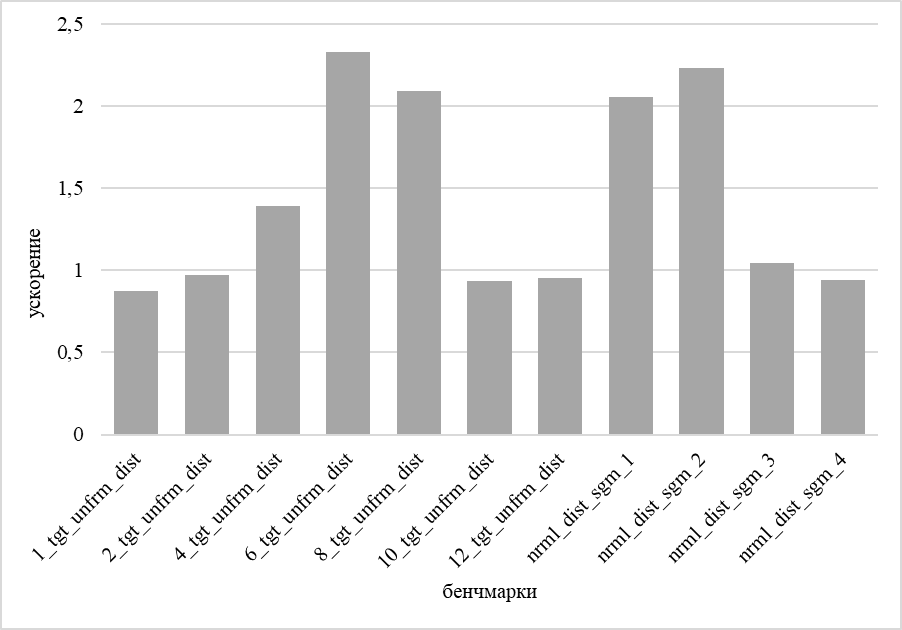
\includegraphics[scale=0.6]{PNG/ICP2}
	}
	\caption{Результаты замеров производительности динамического подхода в зависимости от распределения количества целевых адресов.}\label{fig:ICP2}
\end{figure}


 \section {Разбиение широких инструкций доступа в память} \label{ch2:split_ldp_stp}
Архитектура ARM имеет сложные инструкции, которые выполняют содержат внутри себя несколько простых , например арифметических или логических операций. Такие инструкции позволяют эффективно использовать ресурсы ЦПУ и уменьшают размер кода. Они повышают производительность и сокращают задержку выполнения операций. Однако для использования сложных инструкций необходимо тщательно понимать их функциональность и ограничения, чтобы обеспечить более качественное выполнение программы. Предыдущие исследования \cite{park2019microarchitecture} показали, что разделение 128-битных инструкций чтения из памяти  может улучшить производительность на отдельных тестах. В ходе данного исследования была продолжена эта работа, и было обнаружено, что в двух случаях использование широкого доступа к памяти может снизить производительность.

\begin{figure}[htbp]
	\centering
	\includesvg[width = 400pt, inkscapelatex=false ]{SVG/split_ldr.drawio.svg}
	\caption{Два случая, когда использование широкого доступа в память приводит к замедлению.}
	\label{splitsvg1}
\end{figure}

Один из них (см. рисунок \ref{splitsvg1}) - это хорошо известный невыровненный доступ. Было выявлено, что широкий доступ к памяти должен быть выровнен по его размеру, в противном случае производительность снижается (даже когда речь идет о загрузке 2х независимых регистров). С другой стороны, было показано, что Kunpeng 920 не может быстро обрабатывать зависимости чтения после загрузки в память, если они имеют разные размеры. По всей видимости аппаратная оптимизация пересылки сохраняемого значения (store-to-load forwarding) \cite{shen2013modern} не может быть выполнена в таком случае. Подробный разбор данной ситуации на симуляторе целевой микроархитектуры можно увидеть в главе \ref{p1:optop:sim}. Поэтому было решено разделить широкие доступы к памяти в эмпирически установленном диапазоне.



\begin{figure}[htbp]
	\centering
	\includesvg[width = 300pt, inkscapelatex=false ]{SVG/wide_ldr.svg}
	\caption{Схема алгоритма разделения сложных инструкций.}
	\label{splitsvg2}
\end{figure}

Для решения этой проблемы был разработан алгоритм (см. рисунок \ref{splitsvg2}), который находит инструкцию определения для базового регистра адреса широкой загрузки. Затем алгоритм ищет все использования этого определения, кроме оригинального. Если алгоритм находит сохранение в память с той же базой, то проверяется целесообразность разделения исходного широкого доступа к памяти. Было предположено, что такой подход разумен, если расстояние между загрузкой и сохранением составляет менее 16 инструкций.

 \section {Уменьшение размеров типов переменных}
 Анализ диапазона значений переменных в компиляторе \cite{harrison1977compiler,  simon2008value}  может помочь в удалении избыточных условий, улучшении постоянного распространения, удалении избыточных вычислений и т. д. В результате исследования было выявлено, что анализ диапазона значений GCC все еще имеет недостатки. Прежде всего, текущая оптимизация распространение диапазона значений не способна получать диапазоны из неизменяемых структур данных, что может быть полезно для предварительно вычисленных таблиц. Кроме того, GCC не может изменить размер переменной. Например, если диапазон переменной - $\{0, 1\}$, но пользователь использует тип \textbf{int} для нее, это неоднозначно, для этого можно использовать тип \textbf{boolean}, то же самое касается \textbf{int64\_t} и \textbf{int32\_t}. К сожалению, это не относится к переменным с плавающей точкой, потому что точность может быть потеряна. Производительность на тесте gzip была улучшена.
 
 \section {Векторизация ленивых вычислений}\label{ch2:lcv}
 Ленивые вычисления в языках С/C++ являются частью стандарта языка. Такой подход помогает оптимизировать программы в том смысле, что необходимые вычисления производятся только в тот момент, когда они нужны, а не заранее \cite{cukic2018functional}. Например, в строке (if (pointer \&\& pointer[idx] > 0)) загрузка из памяти гарантированно  не будет выполнена до того момента, как значение указателя не проверится на отличие от нуля. 
 
 Однако такая семантика может приводить к излишним конструкциям, которые в итоге демонстрируют замедление производительности в некоторых случаях.
 Так например в листинге \ref{lcv1} такой подход приводит к замедлению исполнения программы из-за того, что в окно суперскалярного процессора помещается слишком мало инструкций. С помощью метода обратной разработки из главы \ref{p1:optop:reverse} первоначально была произведена замена целевого кода на векторизованный, что показало улучшение производительности, после этого можно было преступать к разработке самой оптимизации.
 
 \begin{ListingEnv}[!h]
 	\captiondelim{ } % разделитель идентификатора с номером от наименования
 	\caption{Кандидат для векторизации ленивых вычислений}\label{lcv1}
 	
 	\begin{Verb}
... code ...
if (arr[len] != const1 || arr[len +1] != const2 
	|| arr[len+2] != const3  || arr[len+3] != const4) {
		/* some code */
	}
... code ...
 	\end{Verb}
 \end{ListingEnv}
 
 Тем не менее векторизация такого участка кода может привести к выходу за границу массива, и в случае выхода за границу выделенной границы памяти может произойти исключительная ситуация seegmentation fault. Чтобы этого избежать предлагается добавить в компилятор знание о страничном устройстве памяти. Обладая этим знанием компилятор может разрешить программе производить чтение за пределами массива, если достоверно известно, что эта страница доступна  программе во время исполнения. Тогда предлагается следующая схема (см рис. \ref{lcv2}):
Перед входом в векторизованный код вставляется проверка на доступность всех ячеек памяти. Т.е  динамически проверяется, что все доступы в память находятся в одной странице памяти. Если условие выполняется, то исполняется векторизованная версия кода, если же нет, то выбирается оригинальная версия.
 
 \begin{figure}[htbp]
 	\centering
 	\includesvg[width = 400pt, inkscapelatex=false ]{SVG/lcv.svg}
 	\caption{Схема векторизации ленивых вычислений].}
 	\label{lcv2}
 \end{figure}
 
 Данный подход вставляет в код одну дополнительную проверку, следовательно в некоторых случаях время исполнения программы может увеличится, однако на целевых тестах такого не наблюдалось, наоборот, наблюдалось ускорение теста gzip.
\section{Слияние хвостов базовых блоков} 

\section{Предзагрузка косвенных доступов в память} \label{opt:prefetch}
Данная оптимизация была выполнена Дьячковым Ильей Леонидовичем, и ожидается, что в своем более подробном варианте оптимизация войдет в его диссертационную работу.  Автор данной диссертации являлся руководителем и соавтором выполненной работы, поэтому позволяет себе кратко рассказать  об оптимизации.  Подробный обзор существующих решений был приведен в главе \ref{pr:prefetch}. 

Анализ аппаратных событий (см. главу \ref{p1:optop:profile}) в приложениях xz и gzip показал большое количество промахов в кэш третьего уровня в горячем цикле. Анализ показал, что в процессе своей работы прилложение очень часто совершает косвенное разыменование указателя. Это значит, что указатель на данные лежит в некой структуре данных (Рисунок \ref{partReview:prefetch3}). Сложность данной работы заключалась в том, что цикл находился глубоко вверху дерева вызовов и косвенная адресация находилась в функции, которая вызывалась косвенным вызовом (по указателю) (Рисунок \ref{optpref1}). 
\begin{figure}[htbp]
	\centering
	\includesvg[width = 300pt, inkscapelatex=false ]{SVG/indirect_prf1.drawio.svg}
	\caption{Граф вызовов внутри основного цикла xz.}
	\label{optpref1}
\end{figure}
Благодаря анализу из главы \ref{opt:devirt} информация о всех кандидатоов для косвенных переходов была уже собрана, оставалось обнаружить цикл, вставить предзагрузку данных и проверку, подобную описанной в главе \ref{ch2:lcv}. Здесь также используется знание о механизме страничной адресации памяти: вставляется динамическая проверка, проверяющая, что необходимая для предзагрузки цепочка загрузок из памяти лежит в доступных страницах. Чтобы разъяснить это утверждение приведем простой пример, который является упрощенной версией кода приложения xz.

  \begin{ListingEnv}[!h]
 	\captiondelim{ } % разделитель идентификатора с номером от наименования
 	\caption{Образец кода для анализа косвенной предзагрузки данных.}\label{ind_pref1}
 	
 	\begin{Verb}
 	typedef struct A
 	{
 		uint8_t *buff;
 		uint32_t *storage;
 		uint32_t a;
 	} A;
 	
 	//foo is calling in a loop somewhere
 	void foo(A *a, uint32_t val)
 	{
 		++a->a;
 		
 		const uint8_t *load_ptr = a->buf +a->a;
 		const uint8_t loaded_value  = load_ptr[0];
 		const uint32_t idx0 = loaded_value & 0x0F;
 		const uint32_t idx1 = loaded_value & 0xF0;
 		const uint32_t idx2 = loaded_value & 0xFF;
 		
 		// indirect stores that we want to prefetch
 		a->storage[idx0] = val;
 		a->storage[idx1] = val;
 		a->storage[idx2] = val;
 	}
 	\end{Verb}
 \end{ListingEnv}
 
  В листинге \ref{ind_pref1} дана функция $foo$, которая вызывается в каком-то другом месте в цикле. Аппаратура очень хорошо справляется с тем, чтобы предсказывать доступ в память $load\_ptr$ так как его изменение происходит чаще всего линейно, с другой стороны предсказание $a->storage[idx]$ дается аппаратуре сложно, потому что она не видит всей картины. Для того чтобы поставить инструкцию $prefetch$ на следующую выгрузку в память $a->storage[idx]$ необходимо знать следующее значение $idx$, которое, к несчастью можно получить только загрузив из памяти $*(a->buf +a->a +1)$ (или еще более далекое значение). Наша цель найти переменную индукции в глобальном цикле ($++a->a$) продвинуть ее, а затем сделать дополнительную выгрузку из памяти, чтобы получить $loaded\_value$ для следующей итерации. В этом месте вставляется проверка, что следующее $loaded\_value$ находится в той же странице памяти, что и текущее и если это так, то производится загрузка из памяти следующего $loaded\_value$ и исполняется инструкция $prefetch$ для следующих выгрузок в память $a->storage[idx0] = val$. Преобразованный код будет выглядеть следующим образом (Листинг \ref{ind_pref2}).
  
    \begin{ListingEnv}[!h]
  	\captiondelim{ } % разделитель идентификатора с номером от наименования
  	\caption{Листинг \ref{ind_pref1} после преобразования.}\label{ind_pref2}
  	
  	\begin{Verb}
	typedef struct A
	{
		uint8_t *buff;
		uint32_t *storage;
		uint32_t a;
	} A;
	
	//foo is calling in a loop somewhere
	void foo(A *a, uint32_t val)
	{

		++a->a;
		
		const uint8_t *load_ptr = a->buf +a->a;
		const uint8_t loaded_value  = load_ptr[0];
		const uint32_t idx0 = loaded_value & 0x0F;
		const uint32_t idx1 = loaded_value & 0xF0;
		const uint32_t idx2 = loaded_value & 0xFF;
		
		a->storage[idx0] = val;
		a->storage[idx1] = val;
		a->storage[idx2] = val;
		
		if (SamePage(a->buf + a->a, a->buf + a->a+1))
		{
			const uint8_t *load_ptr_prf = a->buf +a->a +1;
			const uint8_t loaded_value_prf  = load_ptr_prf[0];
			const uint32_t idx0_prf = loaded_value_prf & 0x0F;
			const uint32_t idx1_prf = loaded_value_prf & 0xF0;
			const uint32_t idx2_prf = loaded_value_prf & 0xFF;
			prefetch_for_store(a->storage + idx0_prf);
			prefetch_for_store(a->storage + idx1_prf);
			prefetch_for_store(a->storage + idx2_prf);
		}
	}
  	\end{Verb}
  \end{ListingEnv}
  
Функция $SamePage$ проверяет, что два адреса находятся в одной и той же странице памяти. Стоит отметить, что такая оптимизация далеко не всегда будет давать производительность, так как определение точного шага индукционной переменной может быть затруднительно и не стоит забывать о том, что наша функция в оригинальном коде вызывается по косвенности, так что нам необходимо каким-то образом учитывать вероятность условных переходов и вызовов функций по указателю. На данном этапе ограничимся статическими вероятностями внутри компилятора GCC, в дальнейшем, в главе \ref{op:mlpgo}, будет показано, как можно улучшить статическое предсказание переходов. 

Представленное решение все еще имеет некоторые ограничения, накладываемые на цепь данных (Data-Flow chain), необходимой для подсчета адреса.
\begin{enumerate}
	\item Цепочка данных может содержать только одно разыменование указателя.
	\item На протяжении всей цепи не должно быть вызовов функций.
	\item Цепь данных не содержит Phi-функций, за исключением головы цикла.
\end{enumerate}

Конечно же данные ограничения являются возможностью для последующих исследований.

\section{Автоматический подбор вероятностей условных переходов}  \label{op:mlpgo}

В главе \ref{pr:pgo} обсуждались компиляторные оптимизации с использованием профиля. В рамках данной работы появилось желание получить улучшение производительности, сходное с оптимизациями с профилем, но без реального исполнения приложения во время компиляции. В компиляторе GCC  существует встроенная возможность компиляции с использованием профиля. Для такого эксперимента необходимо скомпилировать приложение с дополнительной опцией \textbf{-fprofile-generate}, затем запустить исполнение аппликации, после чего перекомпилировать с  дополнительной опцией \textbf{-fprofile-use}. В результате будет получено приложение скомпилированное с использование профиля. Замер производительности показывает среднее увеличение производительности в 5 \% (Таблица \ref{op:pgo1}), однако стоит отметить, что такой запуск практически недостижим в реальной жизни,  так как профиль собирался на тех же входных данных, на которых происходил замер производительности. Тем не менее присутствует значительный потенциал, который хотелось бы использовать.
\begin{table} [htbp]
	\centering
	\begin{threeparttable}% выравнивание подписи по границам таблицы
		\caption{Ускорение приложений CPUBench FP при компиляции с использованием профиля.}\label{op:pgo1}%
		\begin{tabular}{| m{5cm} | m{8cm}l |}
			\hline
			\hline
			\centering \textbf{Приложение}			 & \centering  \textbf{Ускорение} & \\
			\hline
			\centering lightgbm			 & \centering  0.95 & \\
			\hline
			\centering nektar			 & \centering 0.99   & \\
			\hline
			\centering cube			 & \centering 1.00  & \\
			\hline
			\centering openfoam			 & \centering 1.05   & \\
			\hline
			\centering lammps & \centering 1.06   & \\
			\hline
			\centering phenglei & \centering 1.06   & \\
			\hline
			\centering phyml 	& \centering  1.08  & \\
			\hline
			\centering povray 	& \centering  1.08  & \\
			\hline
			\centering gromacs 	& \centering  1.14  & \\
			\hline
			\centering   	& \centering    & \\
			\hline
			\centering Geomean 	& \centering  1.045  & \\
			\hline
			\hline
		\end{tabular}
	\end{threeparttable}
\end{table}

Ранее обсуждалась статья  \cite{rotem2021profile}, в которой была применена техника искусственного профиля. К сожалению, использовать их результат напрямую не получится из-за сильного различия инфраструктуры  GCC и LLVM. Поэтому для начала была предпринята попытка повторить их результат. В качестве набора признаков для каждого условного перехода собирался набор признаков, описанный в таблице \ref{op:pgo_geatures2}. Оптимизация позволяет включить внутри компилятора проходы, которые обычно используются для оптимизаций с профилем (FDO). 

Для сбора обучающей выборки был использован набор программ из пакета ExeBecnh \cite{armengol2022exebench}. Пакет содержит сотни маленьких приложений, которые можно быстро перетранслировать и собрать данные. Процесс сбора данных выглядит следующим образом (рисунок \ref{op:mlpgo1}): Набор обучающих данных компилируется  с использованием своего же профиля и в это время новый проход в компиляторе, названный \textbf{ipa-smart-profile}, собирает различную статическую информацию (таблица \ref{op:pgo_geatures2}) для каждого условного перехода внутри программы. 

\begin{figure}[htbp]
	\centering
	\includesvg[width = 450pt, inkscapelatex=false ]{SVG/FlowMLPGO1.drawio.svg}
	\caption{Сбор данных для тренировки.}
	\label{op:mlpgo1}
\end{figure}

Для обучения используется библиотека \textbf{XGBoost}, которая строит решающие деревья над собранным набором данных, модель сохраняется в бинарном формате, для последующего использования в компиляторе (рисунок \ref{op:mlpgo2}).

\begin{figure}[htbp]
	\centering
	\includesvg[width = 400pt, inkscapelatex=false ]{SVG/FlowMLPGO2.drawio.svg}
	\caption{Тренировка модели.}
	\label{op:mlpgo2}
\end{figure}
Наконец, обученная модель может прогнозировать вероятности  переходов  без использования каких-либо данных профиля, а проход ipa-smart-profile включает оптимизации с профилем. Библиотека \textbf{XGBoost} также имеет C API, который позволяет интегрировать этап прогнозирования в проход без использования \textbf{Python}. Достаточно обучить модель один раз, чтобы потом использовать ее постоянно. Во время выполнения анализ собирает информацию об условных переходах  внутри программы в векторе признаков и передает ее функции \textbf{XGBoost} для прогнозирования.
\begin{figure}[htbp]
	\centering
	\includesvg[width = 400pt, inkscapelatex=false ]{SVG/FlowMLPGO3.drawio.svg}
	\caption{Запуск модели во время компиляции целевого приложения.}
	\label{op:mlpgo3}
\end{figure}

Качество натренированной модели можно оценить при помощи графика \ref{fig:prediction1}. По горизонтальной оси: номер условного перехода в тестовой выборке из пакета ExeBench после сортировки. По вертикальной оси: разница между предсказанной вероятностью с помощью модели и собранной при помощи инструментарии GCC. тем не менее, полученные результаты не оправдали своих ожиданий  (таблица \ref{op:pgo2}). Несмотря на улучшение производительности на тесте \textbf{gromacs} в 15 \%, большинство тестов показало деградацию  производительности. Методу требуется дальнейшее улучшение. Если вернуться к оригинальному исследованию  \cite{rotem2021profile}, то в нем обучение и замер производительности проходил на одних и тех же данных, что в нашей ситуации неприемлемо.  

\begin{figure}[ht]
	\centerfloat{
		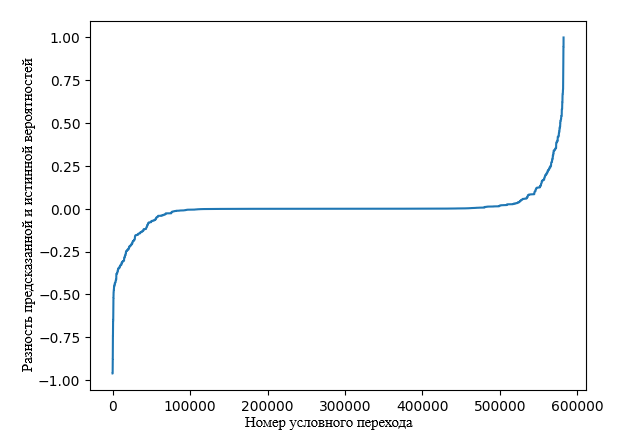
\includegraphics[scale=0.9]{PNG/prediction}
	}
	\caption{S-кривая вероятностей предсказанных переходов на тестовом пакете ExeBench.}\label{fig:prediction1}
\end{figure}


\begin{table} [htbp]
	\centering
	\begin{threeparttable}% выравнивание подписи по границам таблицы
		\caption{Ускорение приложений CPUBench FP при компиляции с использованием предсказанного с помощью решающих деревьев  профиля .}\label{op:pgo2}%
		\begin{tabular}{| m{5cm} | m{8cm}l |}
			\hline
			\hline
			\centering \textbf{Приложение}			 & \centering  \textbf{Ускорение} & \\
			\hline
			\centering phyml			 & \centering  0.80 & \\
			\hline
			\centering cube			 & \centering 0.89   & \\
			\hline
			\centering nektar			 & \centering 0.90  & \\
			\hline
			\centering lightgbm			 & \centering 0.95   & \\
			\hline
			\centering lammps & \centering 0.98   & \\
			\hline
			\centering phenglei & \centering 0.99   & \\
			\hline
			\centering povray 	& \centering  1.00  & \\
			\hline
			\centering openfoam 	& \centering  1.04  & \\
			\hline
			\centering gromacs 	& \centering  1.15  & \\
			\hline
			\centering   	& \centering    & \\
			\hline
			\centering Geomean 	& \centering  0.96  & \\
			\hline
			\hline
		\end{tabular}
	\end{threeparttable}
\end{table}

\section{Выводы по главе и замеры производительности}  \label{results}
В третьей главе  было описано более десяти различных компиляторных оптимизаций и их улучшений, которые были получены после анализа литературы в главе \ref{ch:chReview} и при помощи методологии, описанной в главе \ref{ch:chMethod}. На момент написания диссертации сообществом были приняты оптимизации, описанные в главах \ref{sec:ch2/sect1}, \ref{sec:ch2/sect2}, \ref{opt:devirt}, \ref{ch2:split_ldp_stp}, \ref{ch2:lcv}, \ref{opt:prefetch}. Автор надеется, что остальные оптимизации будут приняты в ближайшем будущем.

Результаты замеров, проведенных в полном соответствии с методологией, описанной в главе \ref{p1:method}, показаны на рисунках \ref{fig:spubench_int_speedup} и \ref{fig:spec_int_speedup}. Можно видеть, что высокие цифры увеличения производительности на тестах пакета CPUBench достигаются за счет значительного ускорения криптографического приложения openSSL. Результаты, полученные на тестах SpecCPU int показывают ускорение за счет теста x264, который также находится в пакете CPUBench.

\begin{figure}[ht]
	\centerfloat{
		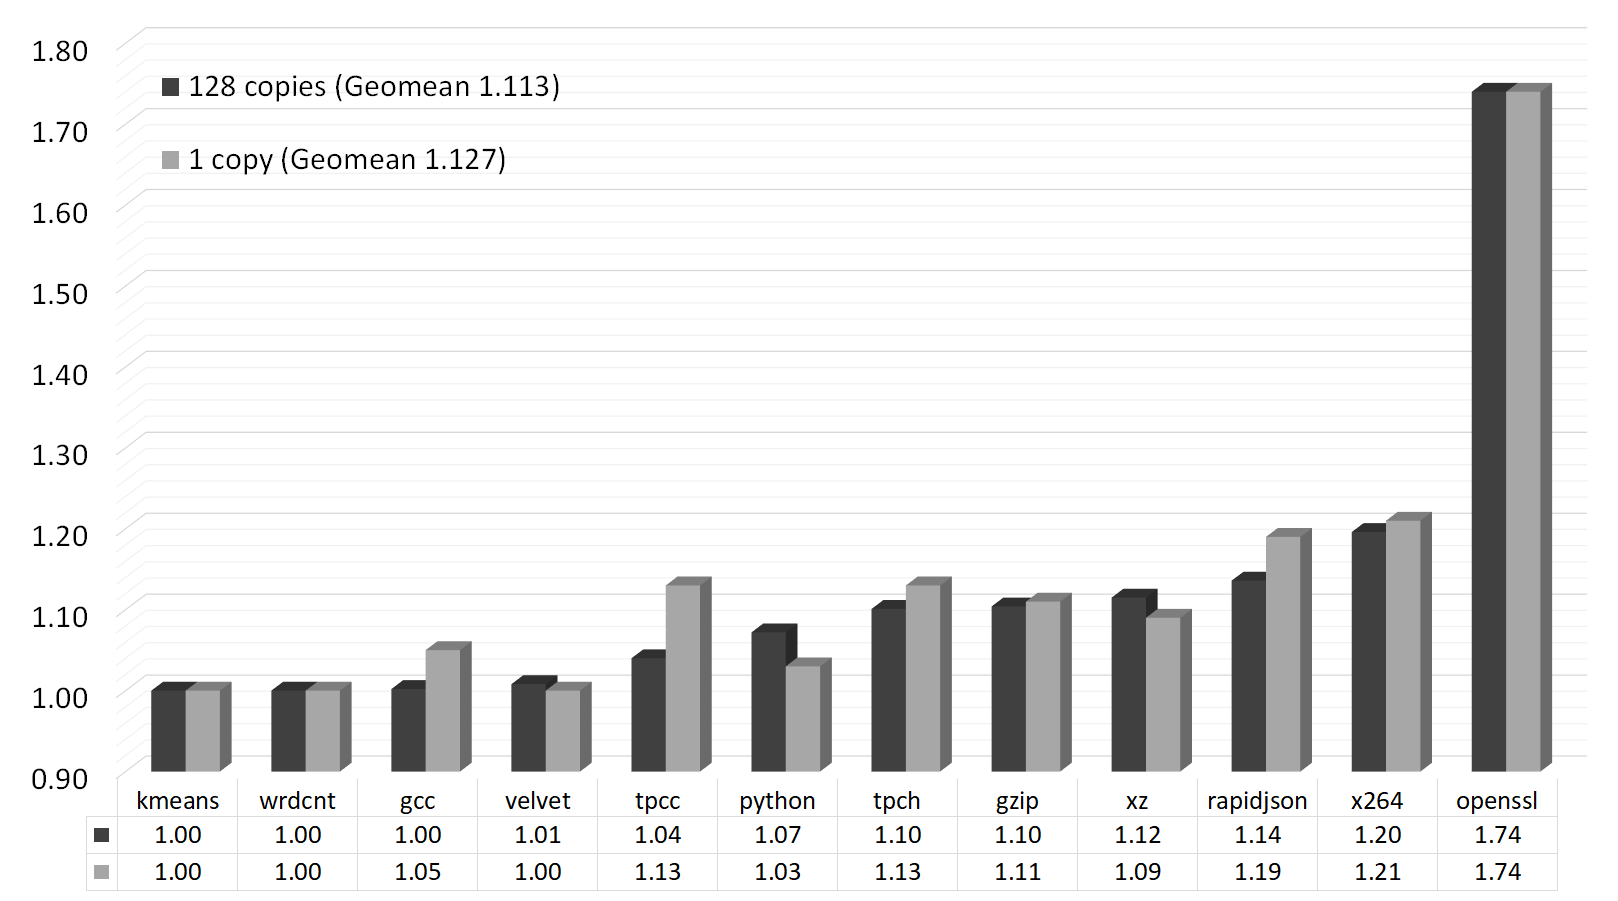
\includegraphics[scale=0.4]{PNG/speedup_combined3.png}
	}
	\caption{Результаты замеров производительности на тестах  пакета CPUBench int.}\label{fig:spubench_int_speedup}
\end{figure}

\begin{figure}[ht]
	\centerfloat{
		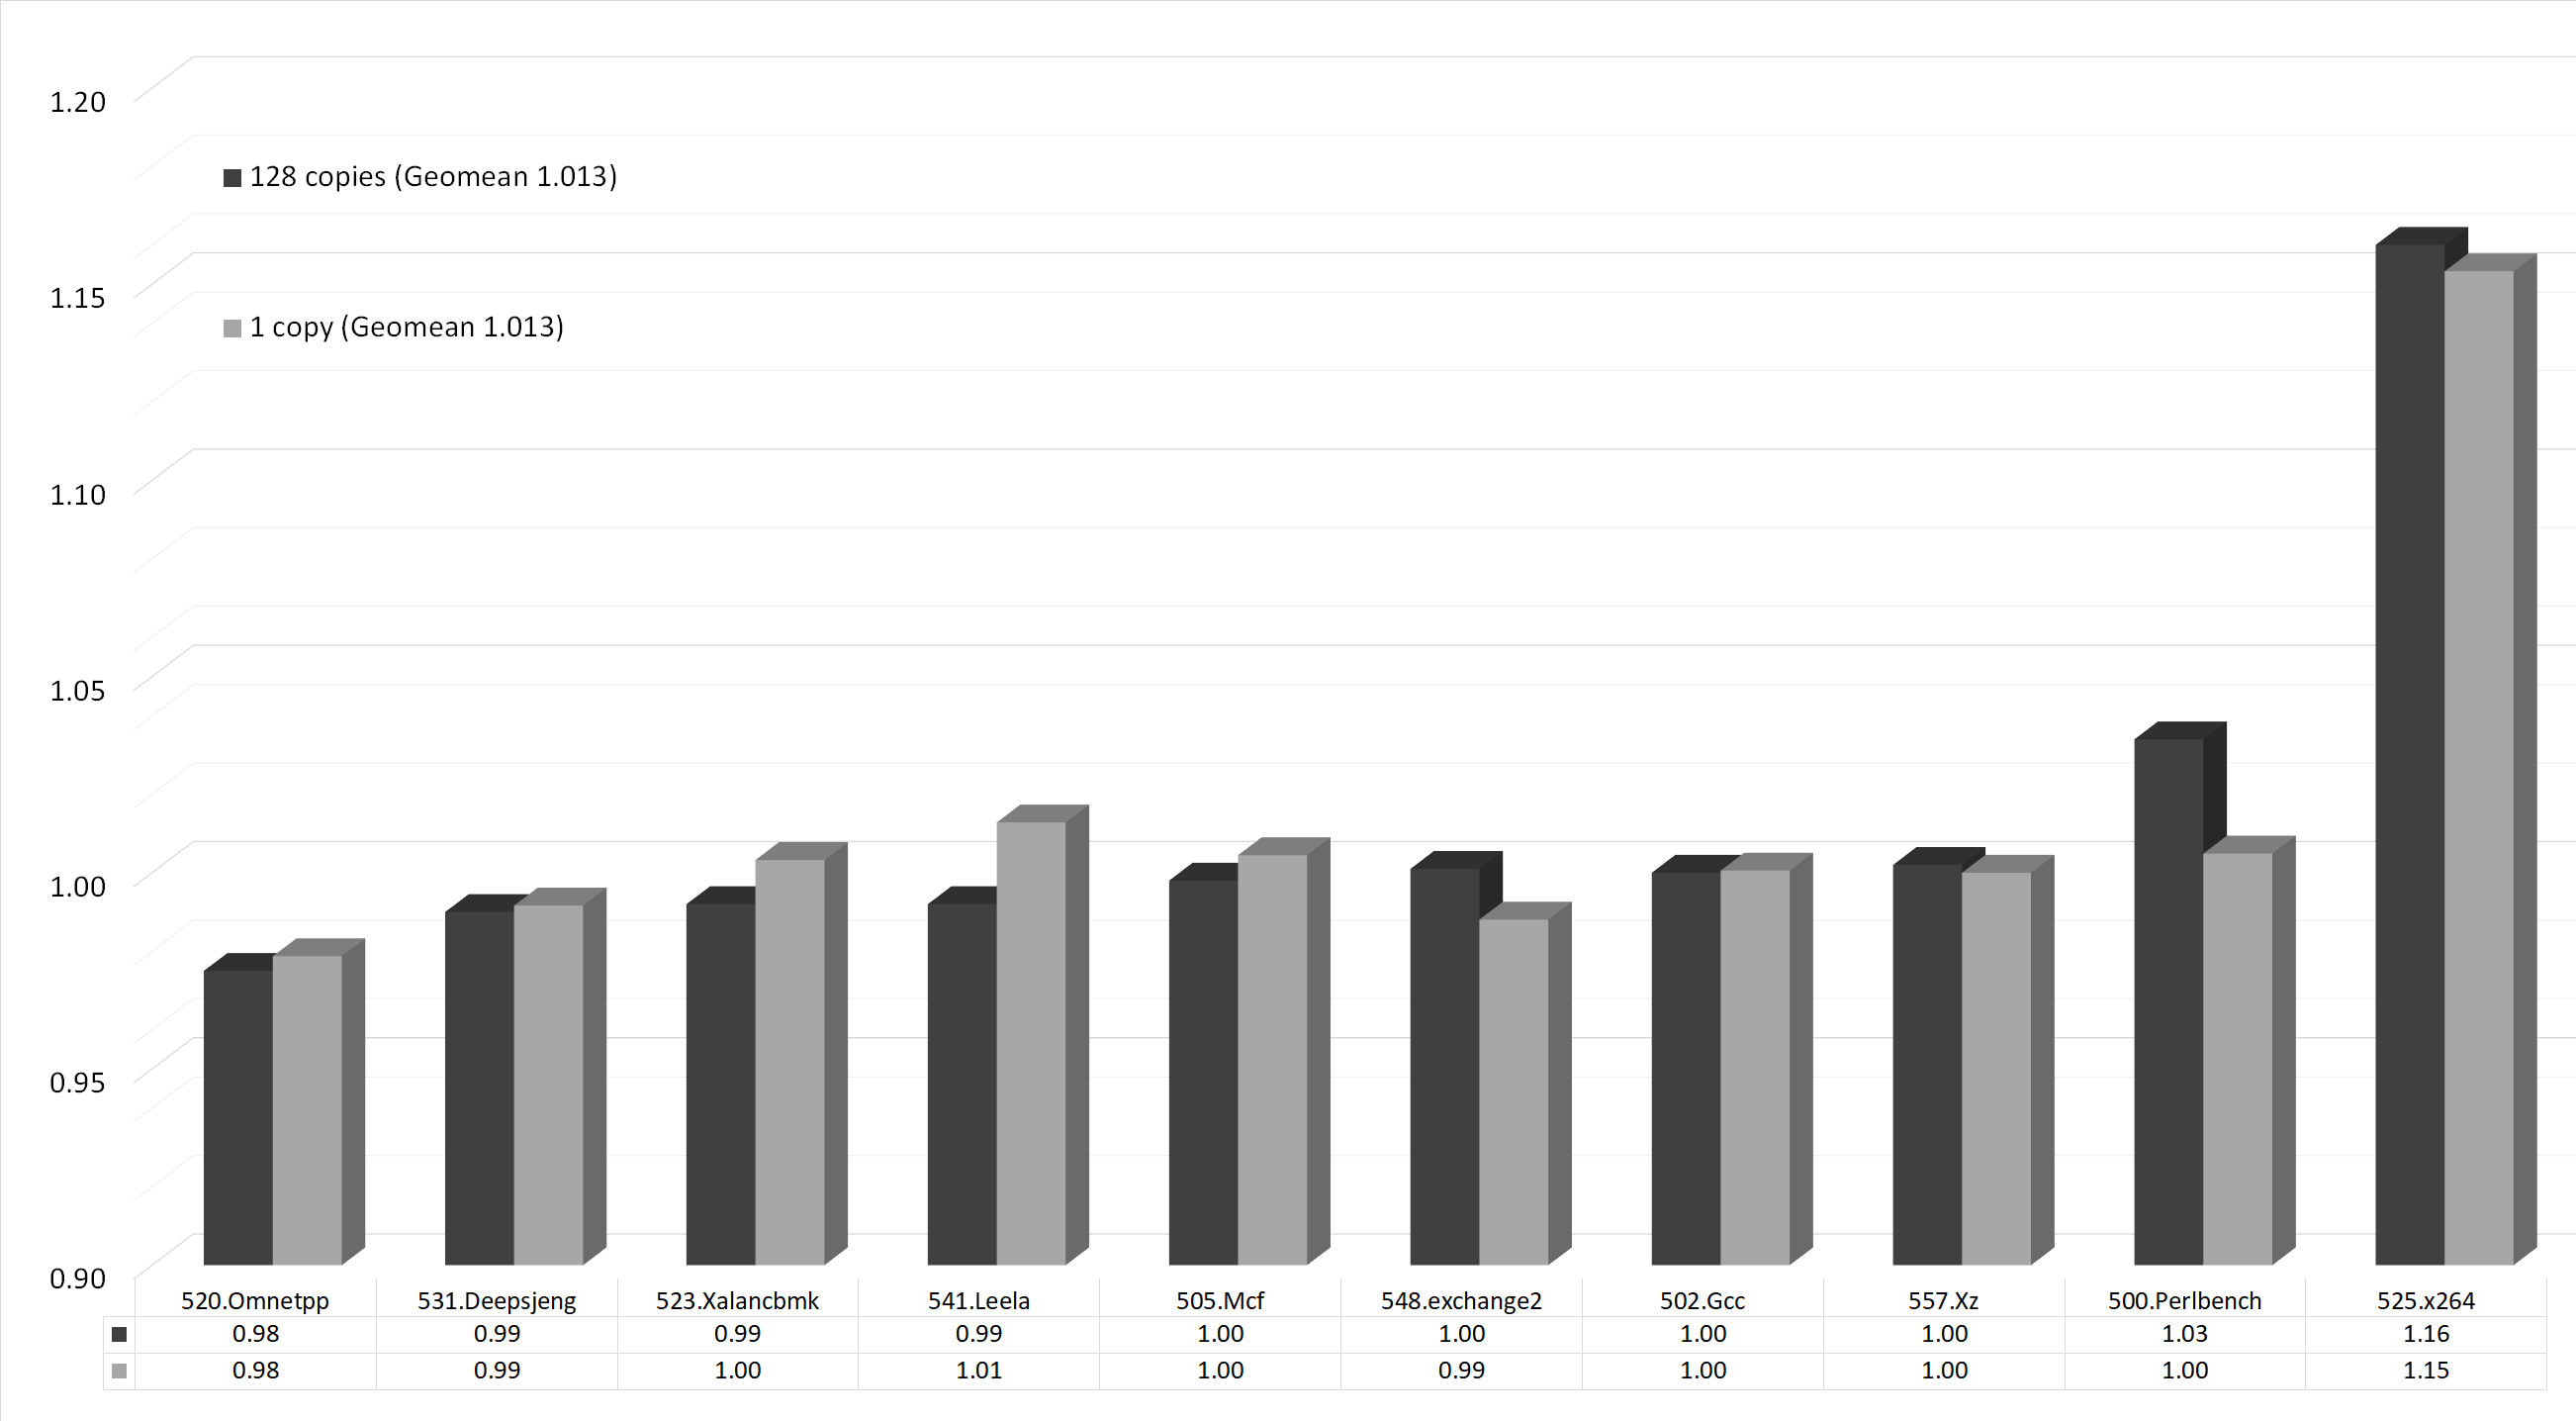
\includegraphics[scale=0.25]{PNG/spec_speedup.png}
	}
	\caption{Результаты замеров производительности на тестах  пакета SpecCPU int}\label{fig:spec_int_speedup}
\end{figure}

